\section{Graphical Design}

Based on our analysis, it turns out that there does not seem to be a relation between the complexity of the graphics, and the impact this has on how 
much fun, the game is or how educating the game is. For this reason 2D graphics has been deemed sufficient for this game. The following section will go 
through the design choices that has been made in terms of the graphical interface of the game, along with justification for why a given choice was made.

\subsection{World Map}

The world map is a hexagon consisting of smaller 'cells' which are also hexagonal. This means that by design the entire field is hexagons in hexagons. 
A cell takes up a single small-hexagon on the field, and as does the various food types a player may encounter. Hexagons were chosen for the map, 
because they add further complexity to the game in terms of 'legal movements' for a cell, relative to if we had chosen squares. Hexagons seemed a good 
design choice, it adds the structure we need as programmers, and it opens up more avenues of play for the players.


\begin{figure}[h]
	\centering
		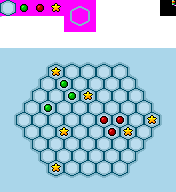
\includegraphics{img/cells_mockup.png}
	\caption{Playing field with cells and food}
	\label{fig:cells_mockup}
\end{figure}

As can be seen by the graphics, food in this example is a star. We have created other mock-ups as well, such as a typical cartoonish ham and an egg. 
Cells are illustrated on the map as green and red 'balls', with green refering to a specific player, and red refering to another player's cells. This 
sort of green and red distinction between the players will be used all throughout the game. The icons chosen for cells and food have been chosen for 
the sole purpose of added clarity, that a player can within reason quickly distinct between food and their cells, and their opponents' cells. By 
chosing different coloring for cells, we feel this is achieved. With all food types taking a none-circular shape or a totally different color-scheme, 
such as a yellow star, it will also help the players distinct between what is food and what are actual player controlled entities.


\subsection{Health Bar}

To give the players, when they compete, a way of getting an idea of how well they are doing in the game, we have decided to design a healthbar at the 
very top of the screen. The idea is that the healthbar will fill with green and red colors, depending on how well the game is going for one of the 
players.

\begin{figure}[h]
	\centering
		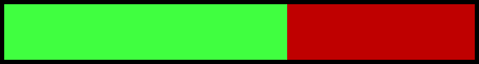
\includegraphics{img/healthbar_example.png}
	\caption{Thre green player has an advantage over the red player}
	\label{fig:healthbar}
\end{figure}

The figure here illustrates how it would look like if the green player has an advantage over the red player during the game. One of the trickier parts 
was to work out, how is an advantage given in the game? Is it based on the number of cells a given player controls? Is it their map position on the 
board - for example; how many food tiles are placed on 'their territorry'? Is it based on how well their algorithm functions compared to the 
opponent's? 


Ultimately we decided that it was enough to simply compare the two players' health points, and determine who had the most life-points. The idea is then 
that the bar will update all throughout the game, and sweep back and forth, depending on which player is doing best throughout a game.

\subsection{Menu Design}

The menu should somehow resemble the design choices that were made for the worldmap, to make the game feel more consistent all throughout. Therefore we 
have worked on a hexagonal design for our menus and the background behind each button. This is an early design, and the menu text may change depending 
on our findings.

\begin{figure}[h]
	\centering
		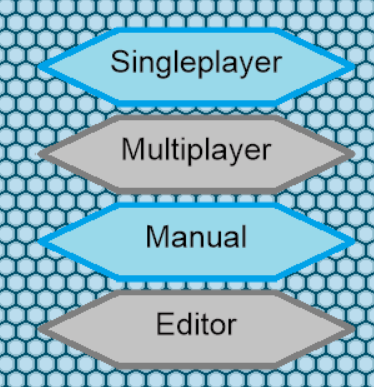
\includegraphics{img/Menu1.png}
	\caption{First menu screen the user sees}
	\label{fig:menu1}
\end{figure}


Notice the hexagonal layer in the background which is the same kind of style used for the worldmap. The color scheme is the same as in the worldmap, 
which is a mixture of light blue and a darker blue color. The options that are not available to the user, for example - what we wind up not 
implementing this semester, or what the user has to unlock by completing challenges, will be drawn in a 'grey' color, to symbolize inactivity as seen 
in other games. Greying out inaccessible parts of the program seems highly used in other types of software, such as windows, LaTeX and various video 
games, so the same convention will be used for this game. Accessible parts of the menu for the user, will be colored in a more vibrant, light-ish blue, 
to distinct them from the grey buttons.
\begin{figure}[h]
	\centering
		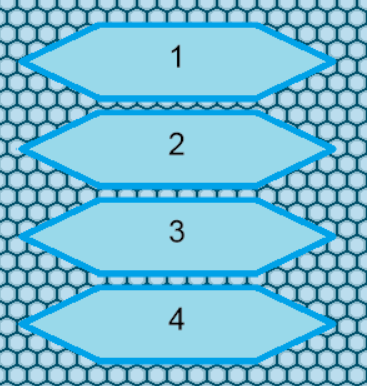
\includegraphics{img/Menu2.png}
	\caption{Second menu screen the user sees}
	\label{fig:menu2}
\end{figure}


When a user clicks a menu button, a new menu will be produced. The menu will represent potential options for the user to take, and they will follow the 
same color scheme as described previously. Examples of what these options could be under Singleplayer, suppose a user could chose a 'Skirmish' kind of 
game, in which their cell competes against a cell AI that we have created. A user may also have access to various programming challenges, aptly named 
'Challenges' in which they have to solve a puzzle - which could function as a sort of tutorial for the user to get into the program. 

It is entirely possible that a menu, would lead to a second, a third, and possibly a fourth.